% RDD - entsprechend der Vorlage von Thomas Lehmann
\documentclass[
   draft=false
  ,paper=a4
  ,twoside=true
  ,fontsize=11pt
  ,headsepline
  ,DIV11
  ,parskip=full+
]{scrartcl} % copied from Thesis Template from HAW


%--------------------------------------- HIER Versionsnummer inkrementieren, 
%------------------------------- auch gerne 0.1.1 ... wenn nur minor changes
\def\ver{0.4}


\usepackage{scrpage2} %Sorgt für erweiterte Formatierungsmöglichkeiten bei KOMA, wie eben Seitenzahlen-Position
\usepackage[ngerman,english]{babel}
\usepackage[T1]{fontenc}
\usepackage[utf8]{inputenc}
\usepackage{longtable}
\usepackage{multirow}
\usepackage{pdfpages} 
\addtokomafont{disposition}{\rmfamily}
\renewcommand{\rmdefault}{ptm}
\renewcommand*{\familydefault}{\rmdefault}

%== Formatierungsschemata ==%
\pagestyle{scrheadings} %Seitenstil festlegen, damit die folgenden Einträge auch wirksam sind
\cfoot{} %center, Fuß, {} = ohne Eintrag
\chead{} %center, Kopf, {} = ohne Eintrag
\ofoot{\pagemark} %Außen, Fuß, Seitenzahl
\ohead{\headmark}

\renewcommand*\titlepagestyle{empty} % unterdrückt seitenzahl
\usepackage[
    left  =7em
   ,right =7em
   ,top   =8em
   ,bottom=8em
]{geometry}


\usepackage{longtable}
\usepackage[german,refpage]{nomencl}

\usepackage{float}

%fürs bilder nach links strecken:
\usepackage{ifthen}
\newcommand {\myspace} 
{%
	\ifthispageodd{
		\hspace*{.25\textwidth}}
		{\hspace*{.25\textwidth}}
}

\usepackage{enumitem}
\usepackage{paralist}
\usepackage{hyperref} % for a better experience
\urlstyle{same}

\hypersetup{
   colorlinks=true % if false - links get colored frames
  ,linkcolor=black % color of tex intern links
  ,urlcolor=blue   % color of url links
}
%\usepackage[ansinew]{inputenc}

\usepackage{amsmath}
\usepackage{graphicx}


\usepackage{array}   % for \newcolumntype macro
\newcolumntype{L}{>{$}l<{$}} % math-mode version of "l" column type
\newcolumntype{R}{>{$}r<{$}} % math-mode version of "r" column type
\newcolumntype{C}{>{$}c<{$}} % math-mode version of "c" column type

\usepackage{listing}
\usepackage{caption}
\usepackage{colortbl}
\definecolor{tabgrey}{rgb}{0.85,0.85,0.85}

\sloppy
\clubpenalty=10000
\widowpenalty=10000
\displaywidowpenalty=10000

\begin{document}
\selectlanguage{ngerman}
\begin{titlepage}
\title{Requirements and Design Documentation \\ (RDD)}
%\subject{subject: Beispiel}
\subtitle{Version \ver \\ \vspace{1em} ESEP – Praktikum – Sommersemester 2017 }
\author{ LANKE \\
\normalsize{
\begin{tabular}{l l l l} 
Hartmann   & Lennart     & 2236791 & \url{Lennart.Hartmann@haw-hamburg.de} \\
Mendel     & Alexander   & 2188808 & \url{Alexander.Mendel@haw-hamburg.de} \\
Eggebrecht & Nils        & 2247014 & \url{Nils.Eggebrecht@haw-hamburg.de} \\
Witte      & Karl-Fabian & 2246435 & \url{Karl-Fabian.Witte@haw-hamburg.de} \\
Veit       & Eduard      & 2227951 &  \url{Eduard.Veit@haw-hamburg.de} \\
\end{tabular}}}
\dedication{
\normalsize{
\begin{tabular}{|l |l |l |p{25em}|}
\multicolumn{4}{l}{ \Large{Änderungshistorie:}} \\
\hline 
\rowcolor{tabgrey} \textbf{Version} & \textbf{Autor} & \textbf{Datum} & \textbf{Anmerkungen/Änderungen} \\
\hline
0.1 &
K.Witte &
04.04.2017 &
Aus der Vorlage (Version 0.5 ) von Prof Lehmann doc2tex, \newline um es in Git besser pflegen zu können \\
\hline
0.1.1 &
K.Witte &
11.04.2017 &
Es wurden Tabellenvorlagen für die Requirements und Use Cases hinzugefügt (Wave und Kite lvl)\\ 
\hline
0.1.2 &
A. Mendel &
10.05.2017 &
Komponentendiagramm der Architektur und Beschreibung\\ 
\hline
0.1.3 &
A. Mendel &
11.05.2017 &
Use Case Aktivitätsdiagramme eingepflegt\\ 
\hline
0.2 &
N. Eggebrecht &
01.07.2017 &
Relogger (Nachtrag von einem anderen) \\
\hline 
0.2.1 &
A. Mendel &
30.07.2017 &
Diverses (Nachtrag von einem anderen)\\
\hline
0.3 &
L. Hartmann &
2.07.2017 &
Finale Steuerung beschrieben\\ 
\hline
0.4 &
K.Witte &
02.07.2017 &
ProfileDetection, Serial, Layer, new Architecture\\
\hline
\end{tabular}
}}
\date{Hamburg, den \today }

\maketitle
\end{titlepage}
\newpage
 

\setcounter{page}{1}
\flushleft

\pagenumbering{roman}
%\begin{abstract}
%Dieses RDD Template stellt eine grobe Struktur des Dokuments dar. 
%Sie können es (fast) nach Belieben verändern.
%Der rot-kursive Text soll durch Ihren Text ersetzt werden.
%Bitte aktualisieren sie bei jeder Meilenstein-Abnahme das Inhaltsverzeichnis.
%\end{abstract}

\tableofcontents
\newpage

%\begin{figure}[H]
%	\label{fig:nobody}
%  	\centering
%    \includegraphics[width=\textwidth]{./IMG/surprise.png}
%    \caption[short Name]{Description}
%\end{figure}


\pagenumbering {arabic}
\section{Teamorganisation}
Teamorganisation:

Die Teamorganisation hat sich im Laufe des Projekts stets dem Entwicklungsfortschritt angepasst.\newline 
Am Anfang des Projekts stand jede Woche ein fester Termin für ein Treffen mit schriftlichem Protokoll fest. Dabei wurden wichtige Punkte für die Architekturplanung und auch schon Designüberlegungen festgehalten. \newline
Ab etwa der Hälfte des Projekts gab es keine festen Termine und keine festen Protokolle mehr, die Organisation fand hauptsächlich mit einem Kanban-Bord statt und sowieso ständig in direkter Zusammenarbeit.

\subsection{Verantwortlichkeiten}
 
 \begin{longtable}{|p{0.2\textwidth} p{0.2\textwidth} p{0.65\textwidth}|}
	\hline
	\textbf{Mitglied} & \textbf{Rolle} & \textbf{Aufgaben} \\ [5pt]
	\hline
	\endhead
	\hline 
	\endfoot
	
	Lennart Hartmann & Architekt (Scrum-Master) & Der Architekt gibt in der Architekturplanung Richtlinien vor und hält über den agilen Entwicklungsprozess fest, was sich an der Architektur verändert hat.

\\	\hline
	

Alexander Mendel & Dokumentator & Der Dokumentator kümmert sich um die sorgfältigkeit aller schriftlichen Ausarbeitungen, die dem Kunden vorliegen.

\\	\hline

Nils Eggebrecht & Product-Owner & Der Product-Owner legt während des Entwicklungsprozesses fest, in welcher Reihenfolge die Aufgaben bearbeitet werden und wie die Priorisierung ist.
\\	\hline

Karl-Fabian Witte & Hauptentwickler & Der Hauptentwickler entwickelt in Zusammenarbeit mit dem Architekten das Softwaredesign. 

\\ \hline

Eduard Veit & Qualitätsmanager & Der Qualitätsmanager ist für die Einhaltung der Coding-Styles verantwortlich. 

\\ \hline



\end{longtable}


%Bennen sie Verantwortliche innerhalb des Projekts (Projektleiter, Tester, Implementierer, etc.). Auch hier ist eine Listen- oder Tabellendarstellung angebracht.
\subsection{Absprachen}

Der Architekt, Herr Hartmann, war im Laufe des Projekts der Hauptansprechpartner für alle Designfragen und Designentscheidungen. Für die jeweiligen Teilgebiete die von anderen umgesetzt wurden, waren entsprechend die Unterteams oder Einzelpersonen verantwortlich. Die Kommunikation lief entweder mündlich in den Räumlichkeiten der Hochschule ab oder sonst intensiv über einen Mobile-Messanger. Für sonstige Kommentare stand eine Kanban-Plattform zur Verfügung.

\subsection{Repository-Konzept}
Das Repository ist in vier Hauptordner aufgeteilt:
\begin{description}
\item[\fbox{CODE}] 
Hier landet der gesamte Sourcecode. Für jede Architekturschicht gibt es mindestens einen Subordner mit den Untermodulen.
\item[\fbox{DIAGRAM}] In diesem Ordner sind alle \emph{Architektur}-, \emph{Design}- und \emph{Use-Case}-Diagramme.
\item[\fbox{DOC}] In diesem Ordner sind alle Dokumentationen rund um das Projekt, wie \emph{User-Stories}, \emph{How-To's}, \emph{Doxygen} und \emph{RDD} zu finden.
\item[\fbox{PROTOKOLL}] In diesem Ordner sind alle sonstigen \emph{Dokumente}-, \emph{Protokolle}- und \emph{Tabellen}.

\item[Aufteilung der Branches] Auf dem \texttt{master}-Branch wird zu jedem Termin ein funktionierender Stand des Projektes entsprechend der User-Story gepusht. Es gibt einen \texttt{develop}-Branch auf den der aktuellste Entwicklungsstand aller \texttt{feature}-Branches gemerged wird, sobald diese, entsprechend der aktuellen Aufgabe lauffähig sind.

\item[Commit-messages] Die Commitnachrichten sind weitesgehend nach einer im Dokument \texttt{how2git.pdf} (im Repositoryordner ``DOC\textbackslash HOW\_TO\textbackslash'' zu finden) vorgegebenen Syntax verfasst. (Dieses Dokument befindet sich im Anhang)
\end{description}

\section{Projektmanagement}
Es wurde das \texttt{Scrum}-Verfahren der \textbf{Agilen Softwareentwicklung} als Softwareentwicklungsvorgehensmodell festegelegt. Eine genaue Analyse der Aufgabenstellung fand im Laufe des Prozesses statt. Das Team war noch nicht mit der Arbeitsumgebung und der Arbeitsweise vertraut.
\subsection{Prozess}
Ab dem Quality-Gate -- Termin wurden Arbeitspakete, die aus einer User-Story zum nächsten Termin formuliert wurden, als \texttt{Sprints} auf einem \emph{Kanban-Bord} festgehalten.

\subsection{PSP/Zeitplan/Tracking}
Die in das Projekt investierten Arbeitszeiten wurden auf einem \emph{Cloud-Spreadsheet} festgehalten. \newline
Auf dem Online-Kanbanbord wurden Arbeitspakete in \underline{Listen} eingetragen:
\begin{description}
\item[\fbox{Ideen}] 
Hier werden allgemeinnützige Informationen festgehalten, die grundsätzlich für das gesamte Projekt von Relevanz waren. \newline
Es ist eine voraussichtliche Zeiteinschätzung für restliche Termine und das Gesamtprojekt hinterlegt, sowie die etwaige Arbeitszeit pro Woche. \newline
Außerdem ist beschrieben was die festgelegten farblichen Labels für die Arbeitspakete bedeutet.
\item[\fbox{Backlog}] In diese Liste werden neue Arbeitspakete eingetragen, die bis zum nächsten Sprint laut \emph{User-Story} bearbeitet werden sollen.
\item[\fbox{Analyse}] In dieser Liste befinden sich die Arbeitspakete aus dem Backlog und werden analyisert und es wird zu jedem Paket eine \texttt{definition of done} formuliert, die z. B. von einem bereits am Modul arbeitenden Teammitglied geprüft und ggf. ergänzt wird.
\item[\fbox{Realisation}] In diese Liste wird ein Arbeitspaket verschoben, wenn es in der Analyse war. Die bearbeitenden Mitglieder tragen sich für das Arbeitspaket ein. Ist die gesamte Aufgabe oder ein Teil der Aufgabe erledigt wird ein kurzer Kommentar zu dem Arbeitspaket veröffentlicht, der umgangssprachlicher als eine \texttt{Commit-Message} beschreibt, was geschafft wurde. Auch wenn neue Designentscheidungen getroffen wurden, wird zum Arbeitspaket ein Kommentar hinzugefügt, so dass andere Teammitglieder, die diese Designentscheidungen betrifft informiert sind.

\item[\fbox{Review}] Ist ein Arbeitspaket nach der \texttt{definition of done} fertiggestellt, landet es in der Review-Liste. Hier segnet der Product Owner oder ein anderes von ihm delegiertes Teammitglied das Arbeitspaket ab oder es wird korrigiert, falls in der Durchsicht Fehler gefunden wurden.

\item[\fbox{Fertig}] Ist das Arbeitspaket erfolgreich geprüft worden, wird es in die letzte Liste verschoben und ist somit abgeschlossen.

\end{description}



\subsection{Qualitätssicherung} %%hier muss evtl noch ergänzt werden
Grundsätzliche Festlegungen zu Code-Conventions sind im Dokument \texttt{coding\_style} festgehalten (unter ``DOC\textbackslash HOW\_TO\textbackslash''). (siehe Anhang)
Es wurde soweit wie möglich zu zweit an einem Arbeitspaket gearbeitet, also \emph{pair programming} betrieben, um Flüchtigkeitsfehler zu vermeiden. 

%\newpage
\section{Randbedingungen}
\subsection{Entwicklungsumgebung}
Als Entwicklungsumgebung wurde im Labor unter Windows 7 mit QNX-Momentics gearbeitet. ``Zuhause'' bzw. auf dem eigenen Rechner auch auf anderen Betriebssystemen und mit anderen Entwicklungsumgebungen.

\subsection{Werkzeuge}

\begin{description}
\item[QNX Momentics V7/V6.6] 
\item[Codeblocks 16] 
\item[CLion 2017]
\item[NetBeans V8.2] 
\item[Dia 0.9] 
\item[Magic Draw 18.5] 
\end{description}

\subsection{Sprachen}

\begin{description}
\item[C] %??
\item[C++] 

\end{description}

%\newpage
\section{Requirements und Use Cases}
\subsection{Systemebene}
Die Use-Case -- Tabelle befindet sich im Anhang.
%Die Anforderungen aus der Aufgabenstellung sind nicht vollständig. Die Struktur der nachfolgenden Kapitel soll sie bei der Strukturierung der Analyse unterstützen. Dokumentieren Sie die Ergebnisse der Analysen entsprechend.
\subsubsection{Stakeholder}

Die Stakeholder dieses Projektes sind in den zwei Kategorien intern und extern unterteilt. In Tabelle \ref{tab:stakeholder} sind diese mit ihren Interessen aufgelistet.

\begin{table}[htp]
\center
\caption[Stakeholder]{interne und externe Stakeholder des Projekts}
\label{tab:stakeholder}
\begin{tabular}{|p{0.25\linewidth}| p{0.7\linewidth} |}
	\hline 
	%-------------------------- intern
	\rowcolor{tabgrey} 
	\textbf{interne Stakeholder} &
		\textbf{Interessen} \\ \hline
	CEO (Management) &
	\begin{compactitem}[-]
    \item Gewinn
    \item Rufaufwertung der Firma
    \item effiziente und flexible Arbeiter
    \item Einhaltung des Zeitplans
    \item transparenter Einblick in den Entwicklungsprozess
  \end{compactitem} \\ \hline
  
	Developer Team & 
	\begin{compactitem}[-]
	  \item motivierende und sinnvolle Arbeit
    \item Gehalt
    \item gutes Teamklima
  %---------------------------- extern
  \end{compactitem} \\ \hline
		\rowcolor{tabgrey} 
	\textbf{externe Stakeholder} &
		\textbf{Interessen} \\ \hline
		Kunde &
		\begin{compactitem}[-]
		\item Projekt hat geforderte Funktion
    \item Projekt hat gewünscht Qualität 
    \item geringe Kosten
    \item schnelles Ergebnis
    \item Regelmäßige Kontrolle des Projekts (Zwischenstand)
    \item Einflussnahme im Projekt, neue Funktionen fordern
  \end{compactitem} \\ \hline
	Anwender & 
	\begin{compactitem}[-]
    \item einfache Bedienung
    \item hohe Sicherheitsstandards im Betrieb
  \end{compactitem} \\ \hline 
	Wartungsservicekraft & 
	\begin{compactitem}[-]
    \item einfache Wartung
    \item geringe Fehleranfälligkeit
    \item hohe Sicherheitsstandards bei Wartung 
  \end{compactitem} \\ \hline
\end{tabular}		
\end{table}

%\subsubsection{Anforderungen}
%In der Aufgabenstellung sind Anforderungen an das System gestellt. Arbeiten sie diese hier auf und ergänzen sie diese entsprechend der Absprachen mit dem Betreuer. Achten sie auf die entsprechende Atribuierung. 
%Berücksichtigen sie auch mögliche Fehlbedienungen und Fehlverhalten des Systems.
%\subsubsection{Systemkontext}
%Use Cases werden aus einer bestimmten Sicht erstellt. Dokumentieren sie diese mittels Kontextdiagramm oder Use Case Diagramm. Die Use Cases und Test Cases müssen zu der hier verwendeten Nomenklatur konsistent sein.
\subsubsection{Use Cases}
Es sind im folgenden Use-Case -- Aktivitätsdiagramme dargestellt, die den Ablauf verdeutlichen. (Abbildung 1 -8)
%Weiteres: Siehe Anhang (Wavelevel UC, Kundentests)

\begin{figure}[H]
	\label{fig:uc1start}
  	\centering
    \includegraphics [width=0.75\textwidth]{./IMG/UseCase_in_Start_1.png}
    \caption[short Name]{Use Case: Puk im Einlauf}
\end{figure}

\begin{figure}[H]
	\begin{addmargin*}[0cm]{-0.15\textwidth}
	\label{fig:uc2profiling}
  	\centering
    \includegraphics [width=1.3\textwidth, scale=1]{./IMG/UseCase_in_Profing_1.png}
    \caption[short Name]{Use Case: Puk in Höhenmessung (Profiling)}
\end{addmargin*}
\end{figure}

\begin{figure}[H]
\begin{addmargin*}[-2.25cm]{0.1\textwidth}
	\label{fig:uc3slide}
  	\centering
    \includegraphics [width=1.3\textwidth]{./IMG/UseCase_in_Slide1_1.jpg}
    \caption[short Name]{Use Case: Puk (Flach/Typ1/Typ5) in Weiche (Band1)}
\end{addmargin*}
\end{figure}

\begin{figure}[H]
\begin{addmargin*}[-2.25cm]{0.1\textwidth}
	\label{fig:uc3slide}
  	\centering
    \includegraphics [width=1.3\textwidth]{./IMG/UseCase_in_Slide1_2.jpg}
    \caption[short Name]{Use Case: Puk (Bohrung/Metall/Typ2/Typ4) in Weiche (Band1)}
\end{addmargin*}
\end{figure}

\begin{figure}[H]
\begin{addmargin*}[0cm]{-0.16\textwidth}
	\label{fig:uc3slide}
  	\centering
    \includegraphics [width=1.3\textwidth]{./IMG/UseCase_in_Slide2_1.jpg}
    \caption[short Name]{Use Case: Puk (Bohrung/Metall/Typ2/Typ4) in Weiche (Band2)}
\end{addmargin*}
\end{figure}

\begin{figure}[H]
\begin{addmargin*}[-2.3cm]{-0.1\textwidth}
	\label{fig:uc3slide}
  	\centering
    \includegraphics [width=1.3\textwidth]{./IMG/UseCase_in_Outrun_1.png}
    \caption[short Name]{Use Case: Rutsche von Band1 voll oder Puk Typ2/Typ4 im Auslauf (Band1)}
\end{addmargin*}
\end{figure}

\begin{figure}[H]
\begin{addmargin*}[-2.3cm]{-0.15\textwidth}
	\label{fig:uc3slide}
  	\centering
    \includegraphics [width=1.3\textwidth]{./IMG/UseCase_in_Outrun_2.png}
    \caption[short Name]{Use Case: Puk entspricht der Sequenz (Band1)}
\end{addmargin*}
\end{figure}

\begin{figure}[H]
\begin{addmargin*}[-2.2cm]{-0.1\textwidth}
	\label{fig:uc3slide}
  	\centering
    \includegraphics [width=1.3\textwidth]{./IMG/UseCase_in_Outrun_3.png}
    \caption[short Name]{Use Case: Puk entspricht der Sequenz (Band2)}
\end{addmargin*}
\end{figure}

%\subsection{Systemanalyse}
%Ihr technisches System hat aus Sicht der Software bestimmte Eigenschaften. Was muss man für die Entwicklung der Software in Struktur, %Schnittstellen, Verhalten und an Besonderheiten wissen? Wählen sie eine Kapitelstruktur, die am besten zur Dokumentation ihrer Ergebnisse% geeignet ist.
%\subsection{Softwareebene}
%\begin{table}[hpt]
%\caption{WAVE LVL USE CASE}
%\label{tab:usecase_wave}
%\begin{tabular}{|p{0.3\linewidth}| p{0.7\linewidth} |}
%	\hline 
%	\rowcolor{tabgrey} \textbf{Name} & \textbf{DER USE CASE NAME (Subjekt + Verb)} \\
%	\hline

%	Akteur & 
%		Wer initiiert die Aktion / Aktivität \\
%	Auslösendes Ereignis &
%		Trigger-Ereignis \\ \hline
%	Kurzbeschreibung & 
%		Informell \\ \hline
%	Vorbedingungen & 
%		Anforderung an globalen Zustand, Werte von Parametern o.ä. \\ \hline
%	Essentielle Schritte &
%		\begin{tabular}{|p{0.4\linewidth}|p{0.52\linewidth}|}
%		\hline
%			\rowcolor{tabgrey} \textbf{Intention \newline der Systemumgebung} & \textbf{Reaktion des Systems} \\ \hline \rowcolor{white}
%
%			Schritt 1: Akteur + Event &
%				Reaktion 1 \\ \hline
%			... &
%				...\\ \hline
%		\end{tabular} \\ \hline
%	
%	Ausnahmefälle &
%		Später einfügen, Initial nur Normalverhalten \\ \hline
%	Nachbedingungen & 
%		... \\ \hline
%	Zeitverhalten &
%		Wenn relevant \\ \hline
%	Verfügbarkeit & 
%		So etwas wie erwartete / notwendige MTBF o.ä. \\ \hline
%	Fragen/Kommentare &
%		Als Merkzetten, Diskussionsgrundlage \\ \hline
%\end{tabular}
%\end{table}

%Tabelle  \ref{tab:usecase_wave} wird mit dem table label im reftag referenziert. 
%\begin{verbatim}
% \ref{tab:usecase_wave}
% allgemein: \ref{table \label}
%\end{verbatim}

%Sie sollen Software für die Steuerung des technischen Systems erstellen. Aus den Anforderungen auf der Systemebene und der Systemanalyse ergeben sich Anforderungen für Ihre Software. Insbesondere wird sich die Software der beiden Anlagenteile in einigen Punkten unterscheiden. Dokumentieren sie hier die Anforderungen, die sich speziell für die Software ergeben haben.
\subsubsection{Systemkontext}

\begin{description}
\item[\fbox{HAL}] 
\emph{(Hardware Abstraction Layer)} Hierzu gehören\newline Sensoren: Lichtschranken, Metaldetektor, Höhenmessungssensor, Bedientasten \newline und Aktoren: Warnleuchten, LEDs, Laufbandmotor und Weiche.
\item[\fbox{Serielle Schnittstelle}] Kommunikation zwischen Gemebox 1 und 2: \newline Packettypen: System-Status-Updates oder Pukdaten.
\item[\fbox{HDI}]\emph{(Human-Device Interface)} Die Schnittstelle zur Konsolenausgabe und Konsoleneingabe.

\end{description}


\subsubsection{Anforderungen}
%Welche wesentlichen Anforderungen ergeben sich aus den Systemanforderungen für ihre Software? Achten sie auf die entsprechende Attribuierung. Berücksichtigen sie auch mögliche Fehlbedienungen und Fehlverhalten des Systems.

\begin{figure}[H]
	\centering
	\includegraphics[width=1.0\linewidth]{./IMG/Puks}
	\caption{Puks}
	\label{fig:Puks}
\end{figure}

\begin{figure}[H]
	\centering
	\includegraphics[width=1.0\linewidth]{./IMG/Leuchten}
	\caption{Leuchten}
	\label{fig:Leuchten}
\end{figure}

%\newpage
\section{Design} 
%Anmerkung: Die Implementierung MUSS zu Ihrem Design-Modell konsistent sein. 
%Strukturen, Verhalten und Bezeichner im Code müssen mit dem Modell 
%übereinstimmen. Daher ist ein wohlüberlegtes Design wichtig.

\begin{figure}[H]
	\label{fig:nobody}
  	\centering
    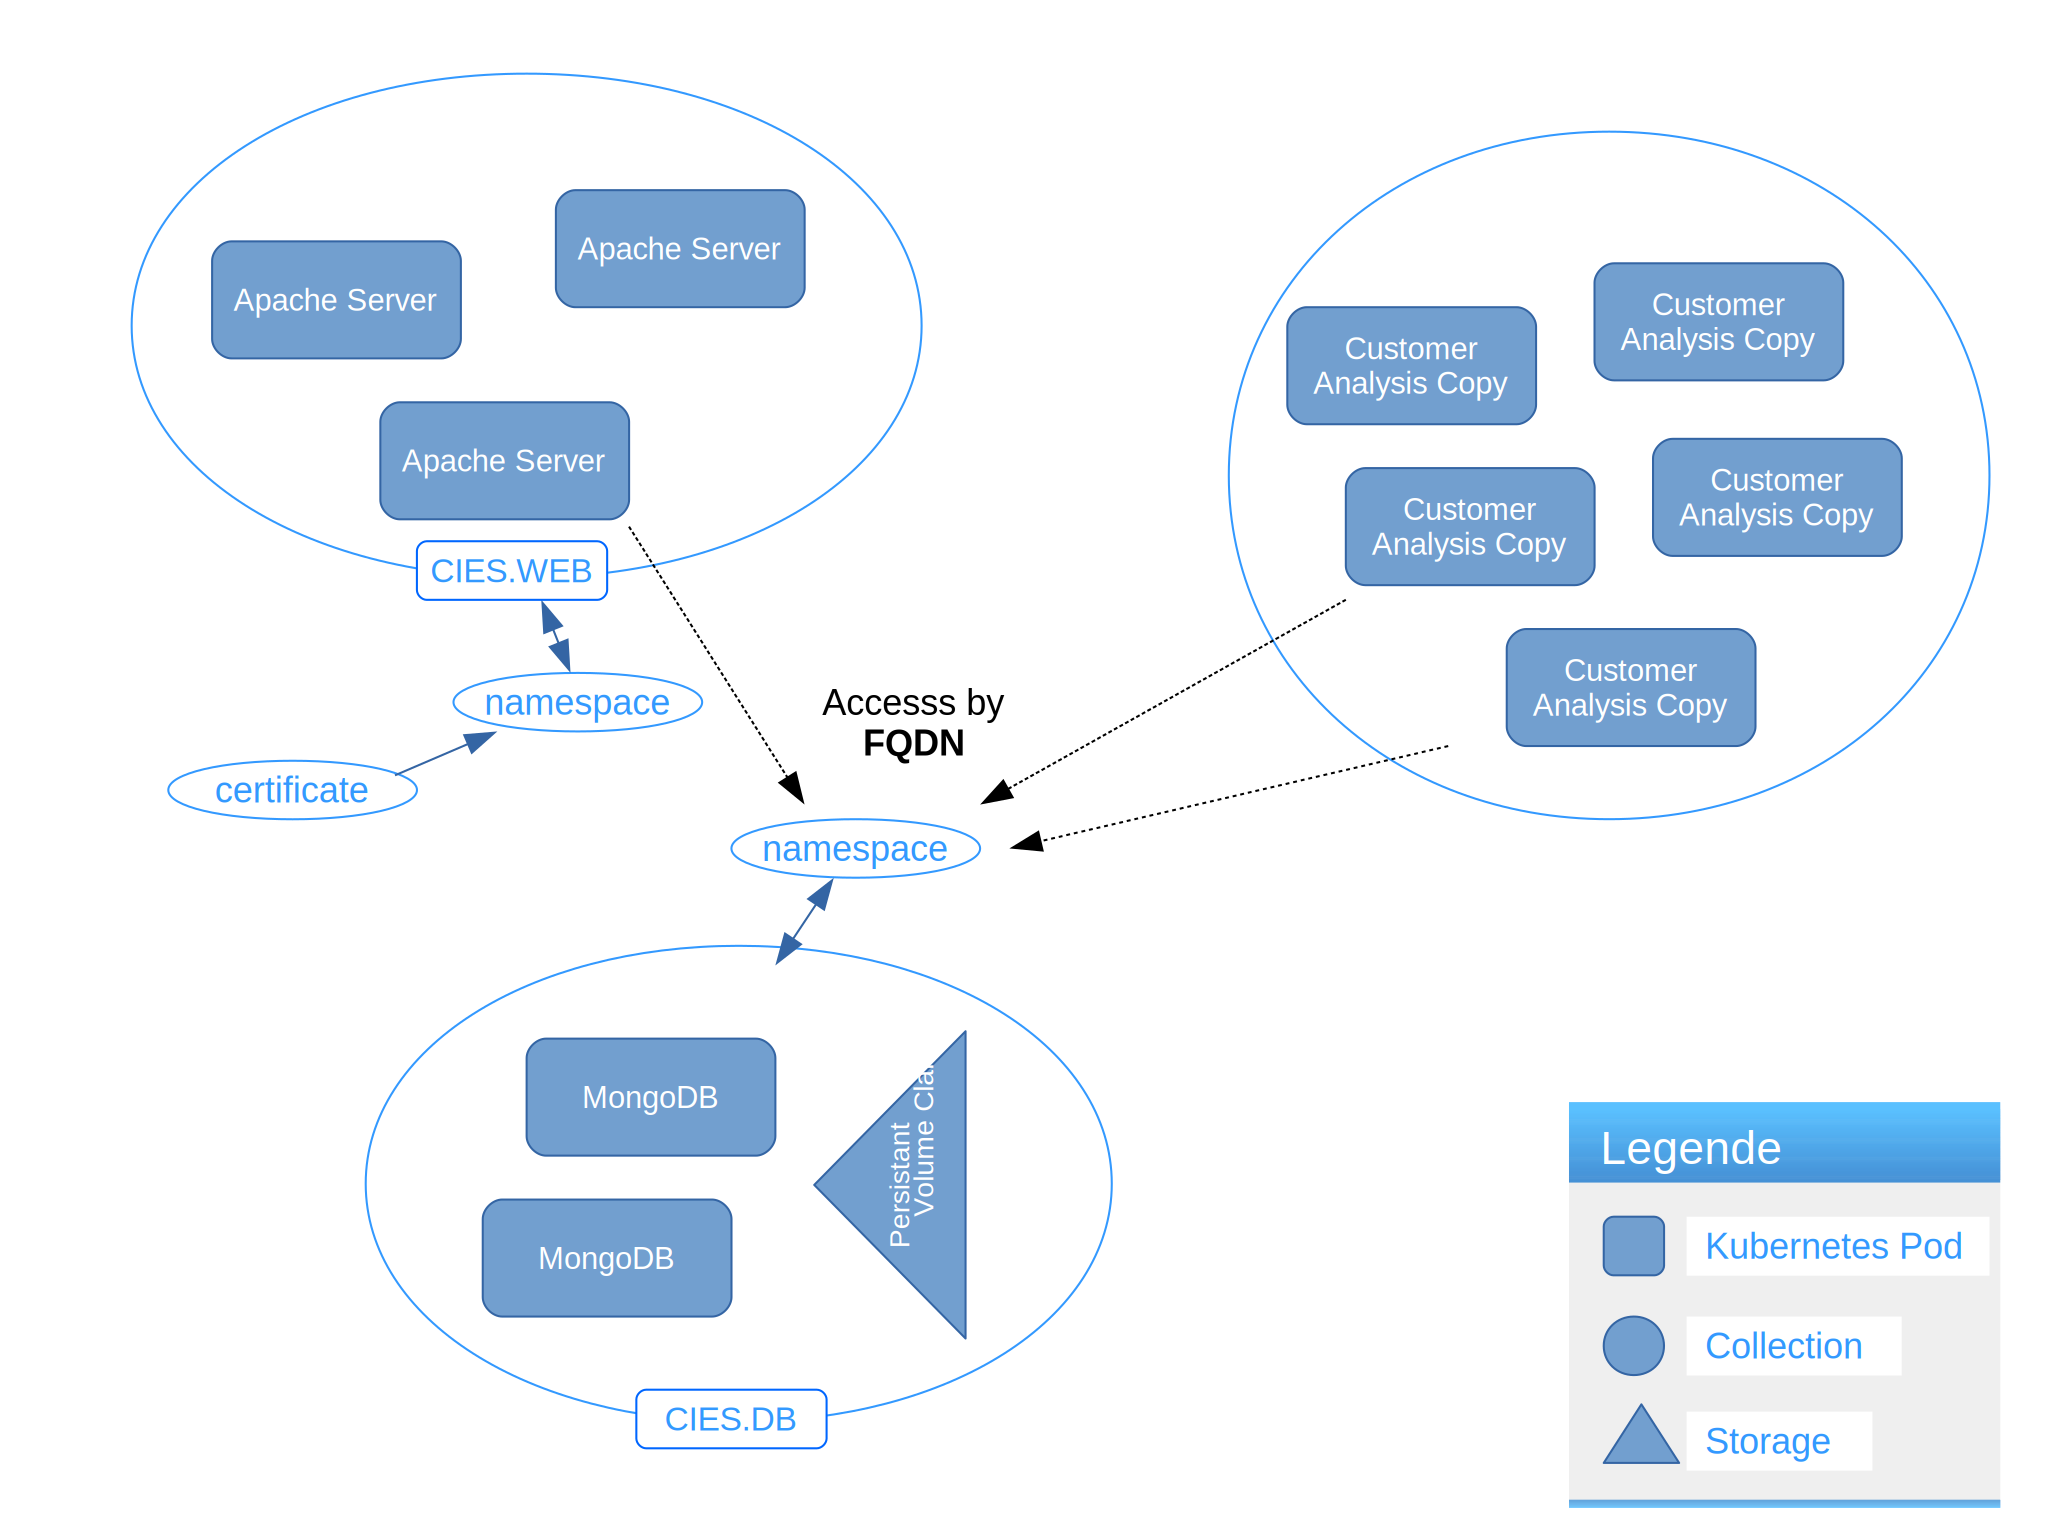
\includegraphics [width=\textwidth, angle=90, scale=1.45]{./IMG/Architektur.png}
    \caption[short Name]{Komponentendiagramm der Architektur}
\end{figure}


\subsection{System Architektur}

\textbf{Übersicht über die Architektur} \newline
Die Architektur ist gemäß der Aufgabenbereiche in drei Schichten ausgelegt. Die Kommunikation zwischen diesen geschieht über \textbf{Pulse Messages}. Hierbei stehen 8 Bit zur Übermittlung von Instruktionen als \texttt{enum} zur Verfügung, sowie 32 Bit, welche zum übergeben der Referenz auf zu manipulierende Daten genutzt werden. Ein blockierendes Verhalten wird somit vermieden.
\newline
\newline
\textbf{HAL}\newline
Die \textbf{HAL} (Hardware Abstraction Layer) abstrahiert die Hardware des Förderbandes, indem sie zwischen \texttt{enum} und Belegungen der Kontroll-Register der für die Ports A-C genutzten I/O-Karten übersetzt. 
Die Komponente \texttt{Sensors} reagiert auf Digitale Inputs, indem sie bei Updates die geänderten Bits in einer ISR identifiziert und der Kontrollkomponente (\textbf{MCL}) deren Semantik in Form eines Signalcodes übermittelt. Sie ist insbesondere für die Erkennung gedrückter Buttons, Metall-Erkennung und Pegelwechseln an Lichtschranken zuständig.
Der \texttt{Dispatcher} hingegen wandelt von der \textbf{MCL} eingehende Kontrollcodes und steuert mit der Komponente \texttt{Aktoren} durch Überschreiben der zuständigen Kontrollregister die Aktorik an.
Die Komponente \emph{Profiling} wird ebenfalls vom \texttt{Dispatcher} angesteuert, nimmt aber in so Fern eine Sonderstellung ein, als sie Autonom durch wiederholte Interaktion mit der analogen I/O-Schnittstelle ein Profil bestimmt und dessen Erkennungscode in als Referenz erhaltene Daten einträgt.

\textbf{MCL}\newline
Diese \textbf{MCL} (Master Control Layer) steuert und überwacht alle Abläufe der Anlage. Sie hält und verwaltet die Daten und Timer und regelt mit Pulse Messages alle angrenzenden Schichten.
Die Komponente \texttt{Dispatcher} verarbeitet alle Eingehenden Pulse Messages, indem sie Transitionen der \textbf{FSM} steuert. Sie reagiert sowohl auf Signale anderer Schichten, als auch auf abgelaufene Software-Timer, die über den über einen gemeinsamen \texttt{Channel} eingehen.\newline
\newline
Die \textbf{FSM} (Finite State Machines) hält den aktuellen Betriebszustand der Anlage und bestimmt ob und in welcher Weise auf Eingaben reagiert wird. Die zugehörigen Funktionsaufrufe steuern Timer und Komponenten der eigenen Schicht und schicken Pulse an angrenzende Schichten.
Der \texttt{TimerManager} erlaubt das Beanspruchen und Stoppen von Timern.  Bei Initialisierung kann eine bestimmte Strecke oder Dauer bis zum Interrupt festgelegt werden. Um auf Änderungen der Geschwindigkeit des Förderbandes zu reagieren, können darüber hinaus alle im Modus „Weg“ arbeitenden Timer gleichzeitig neu parametrisiert werden.\newline
Die Komponente \texttt{PukManager} verwaltet die auf der Anlage befindlichen Puks als Struktur in einer \textbf{Liste}. Sie hat Referenzen auf die als Nächstes in den für Zugriffe relevanten Positionen erwarteten Puks, sodass die Verteilung auf der Anlage mit minimalem Aufwand die abgebildet werden kann. Sie allein ist für Instanziierung und Löschung zuständig. Wir verwenden das \emph{Shared-Memory-Konzept}. Innerhalb einer Anlage werden Referenzen verwendet. Kopiert wird nur beim Transfer auf die zweite Anlage.
Die individuelle Puk-Struktur enthält sämtliche zum physikalischen Objekt erfassten Daten. Sie enthält darüber hinaus Referenzen auf zugehörige minimal- und maximal-Timer für die Erwartete Dauer bis zur nächsten erfassbaren Position sowie eine vorläufige Entscheidung über die ggf. zu nutzende Weiche zum Ausleiten.\newline
Der \texttt{SerialManager} erlaubt den \textbf{FSMs} mehrerer Anlagen zu kommunizieren, um Benachrichtigungen über Fehlerzustände auszutauschen und blockierte Eingänge/Rutschen zu melden. Er ermöglicht ferner beim Transfer von Puks zum angrenzenden Band die korrespondierende Datenstruktur zu übergeben.\newline
Der \texttt{HDI-Manager} dient der Ansteuerung  der \textbf{HDI}. Er soll insbesondere Puk-Strukturen und Messwerte der Kalibrierung  für die Anzeige aufbereiten.
\newline
\textbf{HDI}\newline
Die Human Device Interface - Layer steuert die QNX-Konsole. Neben der Anzeige von Daten soll sie gegebenenfalls selbstständig die Semantik Tastatureingaben selbständig identifizieren und \textbf{MCL} per Pulse benachrichtigen können.

\subsubsection{Nachtrag}
Da der HDI eine sehr kleine Funktion in unserem Design hat, wurde dieser Layer in den MclLayer mit eingebunden. 
Somit erhalten wir eine Zweilayer Struktur.
Die neue Architektur ist in Abbildung \ref{fig:newArch} dargestellt.

\begin{figure}[htp]
  	\centering
    \includegraphics[width=\textwidth]{./IMG/newArch.png}
    \caption[neue Zweischichten Arch]{ZweischichtenArchtiektur: kräftige, gerade Pfeile: Kommunikation über PulseMessages (Channel), dünne,runde Pfeile: Funktionsaufrufe. Dies ist eine vereinfachung der Architektur und sollte als Componentendiagramm interpretiert werden. Dabei ist der ober LAyer die MCL. Die Hal und die Serial ist im Anhand als Klassendiagramm dargestellt und somit wird hier dadrauf verzichtet. Zwischen den Komponenten, welche keine FSMs sind (Controller, HDI/PukManager), wird ebenfalls über Funktionsaufrufen kommuniziert. }
     \label{fig:newArch}
\end{figure}

Der Vorteil dieser Architektur ist die quasi (linare) Unabhängigkeit der Signale zu den Statemaschienes, sodass es einfach ist, eine neue Messstation einzubauen.
Man muss nur entsprechend eine neue Statemaschine  hinzufügen und die Zulieferer entsprechend erweitern.

FSM-Modelle: siehe Anhang(State Machines)
Hal und Serial: Klassendiagramme: siehe Anhang(Hal/Serial)


%\subsection{Datenmodellierung}
%Bestimmen sie das Datenmodell und dokumentieren sie es hier mit Hilfe von UML Klassendiagrammen unter Beachtung der Designprinzipien. Die Modelle können mit Hilfe eines UML-Tools erstellt werden. Hier ist dann ein Übersichtsbild einzufügen.
%Geben sie eine kurze textuelle Beschreibung des Datenmodells und deren wichtigsten Klassen und Methoden an.
%\subsection{Verhaltensmodellierung}
%Ihre Software muss zur Bearbeitung der Aufgaben ein Verhalten aufweisen. Überlegen sie sich dieses Verhalten auf Basis der Anforderungen und modellieren sie das Verhalten unter Verwendung von Verhaltensdiagrammen. Sie können für die Spezifikation der Prozess-Lenkung entweder Petri-Netze oder hierarchische Automaten verwenden. Die Modelle können mit Hilfe eines UML-Tools erstellt werden. Hier sind dann kommentierte Übersichtsbilder einzufügen.
% -----------------------------------------------------------------------
\newpage
\section{Implementierung}
%Anmerkung: Nur wichtige Implementierungsdetails sollen hier erklärt werden. Code-Beispiele (snippets) können hier aufgelistet werden, um der Erklärung zu dienen. 
%Anmerkung: Bitte KEINE ganze Programme hierhin kopieren!
\subsection{Wrapping}
Abbildung \ref{fig:thread} und \ref{fig:channel} beschreiben die gewarppten
Funktionen des Threads und QNX-PulseChannels und deren Hilfsklassen, was nötig ist, um folgende Bilder zu verstehen.
Zudem wrden in der statischen Klasse \texttt{mgt} die \texttt{chrono} Bibliothek gewrappt, um mit ihr einfacher den Softwaretimer zu implementieren.
So wurde eine Funktion zum berechnen der Zeitdifferenz \texttt{mgt::elapse(timePoint \&last)} erstellt.   
\begin{figure}[htp]
  	\centering
    \includegraphics[width=\textwidth]{./IMG/thread.png}
    \caption[thread-uml]{Threadwrapper mit seinen Hilfsklassen.}
     \label{fig:thread}
\end{figure}

\begin{figure}[htp]
  	\centering
    \includegraphics[width=\textwidth]{./IMG/channel.png}
    \caption[channel-uml]{Channelwrapper undseine Hilfsklassen}
     \label{fig:channel}
\end{figure}

  
\subsection{Layerconnection und Communication}
Pro Layer existier ein Sigelton Entity Object, welches den Hauptthread der Layer verwaltet (meist Dispatcher) und die Channels der Komunikation hält.
In der Main werden diese Objecte instaziiert und die Layer mit über die Channel miteinander verbunden. Erst wenn das geschehen ist, wird eine entsprechende init Methode ausgefüht, um die hauptThreads und weiterenKlassen zu instanziieren und zu starten. In Abbildung \ref{fig:layer} sind die Klassen in UML dargestellt. 
\begin{figure}[htp]
  	\centering
    \includegraphics[width=\textwidth]{./IMG/layer.png}
    \caption[layer]{layer Klassendiagramm: Die Großen EntityKlassen, um die Layer miteinander zu verbinden und den Layerhauptthread zu verwalten.}
     \label{fig:layer}
\end{figure}
\newline
Die Kommunikation der Layer erfolgt dann über die Channel, welche diese EntitySingeltons haben. Dabei gehört der Channel dem, der auf diesen hörcht.
Die Kommuniktion erfolg dabei auf dem Prinzip der PulseChannel von QNX. Dafür wurde eine vereinfachung der Pulsestruktur gewrappt. \texttt{Pulse\_t} besteht aus einem identifizierungs Code \texttt{code} (8bit) und einem inhaltswert \texttt{value}, welcher als Ganzzahl oder als Pointer verwendet werden kann. In Abbildung \ref{fig:interLayerCom} sind die Interfaces nochmal dargestellt.
\begin{figure}[htp]
  	\centering
    \includegraphics[width=\textwidth]{./IMG/interLayerCom.png}
    \caption[layer]{layer Klassendiagramm: Die Interfaces zuwischen den Layern}
     \label{fig:layer}
\end{figure}
\newline

\subsection{Timer}
Es werden im Code Software-Timer statt Hardware verwendet, da diese einfacher zu implentieren sind und das System ausreichend Ressourcen für diese verfügbar hat. Die Software-Timer werden asynchron verwendet um keine anderen Prozesse zu blockieren. Außerdem ist der Code so weitgehend betriebssystemunabhängig und kann so auch auf anderen Plattformen eingesetzt werden. Da sich alle Timer in der MCL befinden, ist dies auch vorzuziehen. Leichte Ungenauigkeiten der Software-Timer im Zeitverhalten sind aufgrund der Echtzeitanforderungen im halb-Sekunden Bereich unproblematisch.
\newline
Die Grundidee ist der laufende Thread der TimerController, der pro Software-Tackt (Thread schläft eine bestimmte Zeit an Millisekunden) alle verwalteten TimerObjekte, neu berechnet. Die TimerObjecte sind einfache Entitäten, welche, die Daten, wie die abzulaufende Restzeit (\texttt{delta}) und den Typen (Distance oder Zeit Timer). 
Der TimerController wertet diese Informationen aus und berechnet bei jedem Tick die neue Restzeit. Wenn diese abgelaufen ist, wird der ebenfalls im Timer gehaltene Rückgabewert in den Mclhauptchannel geschrieben.
Jedes TimerObjet muss mit der Factoryfunktion \texttt{getTimer()} des TimerControllerObjectes erzeugt werden, damit diese Timer auch von diesem bearbeitet wird. Ein Timer wird neu aufgezogen, indem das entsprechende MCL\_signal in der Methode TimerController::resetTimer(Mcl\_signal ret) verwendet wird. 
% -----------------------------------------------------------------------
\subsection{Interrupts}
In der Hal werden einkommende Signal auf Port B und C entsprechend ausmaskiert und über ausgewertet, ob es sich um eine steigende Flanke handelt oder um eine fallende. Das Ergebinis wird auf das entsprechende MCL\_input\_signal gemappt und nach oben gesendet.

\subsection{Profile Erkennung}
Die Profilerkennung startet beim Eintritt in den Bereicht (unterbrechung der Lichtschranke), misst den Puk von der Mitte bis über den Puk hinaus, wird beendet beim Austreten des Bereiches (Lichtschranke geschlossen) und die ist wie folgt aufgebaut: 
\newline
In der Mcl:
Der ProfileController holt sich den Puk in seinen Speicher und schickt der Hal den Befehl zu Starten der Profilmessng runter.
\newline
In der Hal:
Es wird der AnalogSensorthread aufgeweckt.
Es wird zunächst das Register, in dem sich der akutelle Wert befindet nach den
Hardwarespezifikation ausgelesen. Dann wird ein Medianfaltungsfilter über die letzten fünf Werte gestellt, um die Fluktuation zu minimieren, und dieses Mittel dann an die Mcl bzw den ProfilDetectionController geschickt.
\newline:
In der Mcl:
Dieser sammelt diese Werte in einer Liste von Buckets so, dass immer der Wert mit dem gewichteten Mittel der letzten Werte verglichen wird. Die letzten Werte sind hier werte, die im Tolerancebereich des Mittels lagen. Liegt der Wert im Toleracebereich des Mittels, wird der Zähler für dieses Mittel hochgezählt (und das Mittel wird neu berechnet). Liegt der Wert nicht im Tolleranzbereich, wird ein neuer bucket in die Liste gesetzt und von dort neu verglichen. So erhält man eine zeitlich korretsortierte BucketList. 
Zum Beenden des Samplinvorgangs schickt der ProfileDetectionController einen Stopp Befehl an die Hal.
\newline
In der Hal:
Im AnalogSensorObject wird ein Flag auf true gesetzt, was das Auslesen der Registers unterbricht und eine (Ende der Profilemessung) Nachricht an den ProfileDetectionController schickt. Im Anschluss schickt sich der Thread selber in den Schlaf.
\newline
In der Mcl:
In der Mcl leitet diese Nachricht die Auswertung der Bucketliste ein.
Zuerst wird geckuckt, ob der Zähler der Buckets groß genug ist. Bei zu kleinen Zähler wird dieser Bucket gelöscht, um fallende und steigende Sinussteigung (entstanden durch die Mittelung in der Hal) zu dezimieren. 
Aus den übrigen Werten wird jetzt das Maximum und das Minimum gesucht und damit der die entsprechende Höhe berechnet, denn es wird auch immer die Höhe des Laufbandes selber mit erfasst.
Es wird das Minimum von den Werten abgezogen und alle Werte, die im Tolleranzbereich des Minimums und des Maximums sich befinden, werden aus der Liste gelöscht. Ist die Listengröße 
nur null, so ist der Puk flach. Ist die Größe eins, so ist der Puk gebohrt.
Ist der Puk größer zwei, so muss es ein Bitcodierter sein. 
Die Liste wird in diesem Fall nochmal durch die Höhe minus Tolleranzbereich Ganzzahlig geteilt. Die nun quasi bitcodierte Liste wird nun in eine Ganzzahl umgewandelt und das Ergebnis wird direkt in den Puk geschrieben.
%-.---------------------------------------------------------------------------
\subsection{Serielle Kommunikation}
Die Gemebox hat zwei Serielle Schnittstellen, was hier ausgenutzt wird. Eine Schnittstelle für eingehende Nachrichten und die andere Schnittstelle dient zum Senden von Nachrichten.
Dabei wird wird auf jede gesendete Nachricht im SerielLayer mit einem bestätigendem ACK gewartet. Das Lesen (Empfangen) von ACK ist hierbei Zeitbeschränkt. Beim Überschreiten der Zeit, wird eine Fehlermeldung hoch an die Mcl geschickt.
Das Protokoll ist entsprechend Aufgebaut( siehe hierfür Abbildung \ref{fig:serial} oben rechts im Anhang):
\newline
In der Mcl: (SerialController)
Zuerst wird ein Header gezeugt, welcher die Art der kommenden Infomation 
beschreibt. Eine Referenz des Headers wird mit entsprechenden Code 
(HEADER\_PTR) nach unten geschickt. Das folgende Packet wird im Anschluss entsprechend runtergeschickt. Um Speicherleaks zu vermeiden, werden die Packete oben in Listen verwaltet und wenn ein SEND\_OK gelöscht.
\newline
In der Serial:
Die von der Mcl kommenden Referenzen werden entsprechend einfach über das  Kabel weitergeleitet.
\newline
Beim Empfangen werden die einzelnen Packete, wird ein ACK auf dem gleichen Kabel gesendet und wegen der Natur des Replayloggers, in seine Einzelteile zerlegt und stückweise in die Mcl geschickt.
%----------------------------------------------------------------------------
\subsection{Log and Replay}
Durch das Loggen der eingehenden Signale des Channels vom \textbf{MCL}, kann ein kompletter Ablauf der einmal auf einem Laufband abgelaufen ist, beliebig oft abgespielt werden.
Es wird die aktuelle Systemzeit beim Start des Ablaufs und beim Eingang jedes Signals getrackt. Außerdem wird der Enum- Wert des Signals und der Wert, welcher Sender es in den Channel geschrieben hat, gespeichert.
\newline
Zum abspielen der Datei, muss das Programm neu ausgefüht werden und beim Start des Laufbands über Tastaureingabe angegeben werden, dass der Replay-Modus ausgeführt werden soll und die entsprechende Log- Datei ausgewählt werden.
\newline
Nach der Auswahl der Datei werden die Signale mit dem richtigen Timing, welches durch die Differenzbildung der Zeit, von dem Signal zuvor, berechnet wird, wieder in den Channel vom \textbf{MCL} geschrieben.
% -----------------------------------------------------------------------
\subsection{Steuerung (FSM)}
Die Steuerung des Systems ist durch vier orthogonale Finite State Machines realisiert. Jede dieser FSMs überwacht/steuert das Verhalten, welches durch das physikalische Eintreffen/Fehlen eines Objekts am der State Machine zugeordneten Ort zum definierten Zeitpunkt beabsichtigt ist, indem sie den einer zugehörigen Hardware-Komponente Controller anspricht, eine Transaktion an einen Manager delegiert und/oder Flags im Shared Memory setzt. Letzteres erlaubt es notwendige Informationen über blockierte Rampen/Übergänge sowie Fehlerzustände global verfügbar zu machen.
\newline
\newline
Ein Multiplexer-Modul gewährleistet die korrekte Zuordung der eingehenden Signale. Die Nutzung eines einzigen Channels als Quelle aller transitionen bewirkender Steuersignale gewährleistet eine vollständige Synchronisierung und Pufferung. Alle Transaktionen sind folglich atomar.
\newline
Die Zuständigkeit der aufgrund ihrer erweiterten Funktionalität als EntryManager, ProfileDetectionManager, GateManager und Outletmanager bezeichenten FSM-Module korrespondiert mit den Orten, an denen aufgrund der an der Anlage befindlichen, orthogonal zur Laufrichtung des Bandes ausgerichteten Lichtschranken Informationen über die Position eines Objektes gewonnen werden können.
\newline
Informationen über zwischen Lichtschranken entfernte bzw. zugefügte Objekte werden aus Timeouts gewonnen. Jeder Puk hat zu diesem zweck Referenzen auf zwei Timer deren Dauer bei Verlassen einer Position mit der minimalen/maximalen benötigten Zeit zum erreichen der nächsten feststellbaren Position reinitialisiert wird.
Das Ausbleiben eines Minimal-Timeouts vor Eintreffen eines Objektes wird als Hinzufügen, das Ablaufen des Maximal-Timers als Entfernen eines Objektes interpretiert. 
\newline
Die Laufzeit aller erzeugten Timer kann und bei Änderung der Geschwindigkeit des Laufbandes aufgrund ihrer Erzeugung durch eine spezielle Factory gleichzeitig angepasst werden.
\newline 
\newline
Jeder Automat erfasst an der zugeordneten Position aufgetrende Fehler und ist ebenfalls für deren Auflösung verantwortlich. Da die Anlage im Fehlerfall der Betrieb stoppt und alle Signale serialisiert eingehen, befindet sich stehts nur eine FSM im Fehlerzustand. Die Auflösung erfolgt bei Erkennen des Reset-Signals, welches an alle FSMs witergemeldet wird.
\newline
\newline
Übergeodnete Zustände werden nur durch Fehler auf der seriell verbundenen Anlage, oder durch die Verwendung von Druckknöpfen erreicht. Sie sind so umgesetzt, dass sie durch das Setzen von als Guards agierenden Flags eine Weiterleitung von Signalen an untergeordnete FSMs unterbinden. 
\newline
\newline
Dies betrifft den E-STOP, welcher das System anhält und das Druchlaufen einer vorgegebenen Sequenz von Button-Events erzwingt bevor die reguläre Weiterleitung Signale  wieder aufgenommen wird, die Unterbrechung aufgrund eines Fehlerzustandes auf andererem Band, das das Verhalten Warnleuchten angleicht  und jede Fortsetzung des Betriebs unterbindet, sowie  ein An/Aus, das lediglich den Betrieb unterbricht. 

Weitere Signale, die keine Transition bewirken, aber aufgrund des Entwurfs nach Zuständigkeit zur Verarbeitung ausgewertet werden, sind Benachrichtigungen über eingegange Messwerte. 


% -----------------------------------------------------------------------
\newpage
\section{Testen}
Beim Testen in der Implementierungsphase hat die Funktionsfähigkeit des regulären Betriebsablaufs Priorität. Erst wenn diese gegeben ist sind Fehlerfälle zu berücksichtigen, um die Komplexität bei Problemen gering zu halten. Dieses Vorgehen kann in der Praxis an der Hardware nur bei Vermeidung von gefahrbringenden Zusätänden angenommen werden.
\newline
Die Softwarekomponenten sind zuerst bei der Implementierung durch simulierte Signale zu testen, die innerhalb der HAL definiert und zeitgesteuert ausgeführt, d.h. an Komponenten weitergegeben werden.
\newline
Nach den erfolgreichen Simulations-Tests werden zusammenhängende Komponenten auch an der Hardware getestet.
%\subsection{Testplan}
%Definieren sie Zeitpunkte für die jeweiligen Teststufen in ihrer Projektplanung. Dazu können sie die Meilensteine zu Hilfe nehmen.
\subsection{Abnahmetest}
Schriftlich ausformulierter Abnahmetest: Siehe Anhang \texttt{Abnahmetest}.
\begin{figure}[H]
	\centering
	\includegraphics[width=1.0\linewidth]{./IMG/Betriebsmodi}
	\caption{Betriebsmodi}
	\label{fig:betriebsmodi}
\end{figure}

\begin{figure}[H]
	\centering
	\includegraphics[width=1.0\linewidth]{./IMG/Bandlauf}
	\caption{Bandlauf}
	\label{fig:bandlauf}
\end{figure}

\begin{figure}[H]
	\centering
	\includegraphics[width=1.0\linewidth]{./IMG/Zeitverletzungen}
	\caption{Zeitverletzungen und Log \& Replay}
	\label{fig:zeitverletzungen}
\end{figure}

\subsection{Testprotokolle und Auswertungen}

\begin{center}\underline{\emph{\textbf{letztes Testprotokoll vor Abnahmetest hier einheften.}}}\end{center}

\subsection{Lessons Learned}

Die Bewerkstelligung des Projekts brachte einige Aufgaben mit sich, die bisher niemand im Team bewältigen musste. Zum einen ist der Umfang der Aufgabe deutlich größer und umfasst mehrere Termine und zum anderen ist dementsprechend die Größenordnung des Projekts und der Teams größer als gewohnt.\newline
Die wichtigste Hürde, die zuerst genommen werden musste, war die Organisation in den großen Teams. Die Absprache und Kommunikation bringt einen exponentiell steigenden schwierigkeitsgrad mit sich, wenn man es gewohnt ist, sich mit nur einem Partner abzusprechen.
\newline
Durch die wegweisenden Hinweise der Aufgabenstellung und der Empfehlungen der Professoren und Erfahrungen anderer Studenten wurde der agile Entwicklungsprozess eingeschlagen und der Fokus auf die Modellierung und allgemein ausformulierte Planung der Anforderung gelegt. 
\newline
Da man es nicht in kurzer Zeit schafft einen tiefen Einstieg in die komplexen Anforderungen der Aufgabe zu machen. Viel die Analyse anfangs schwer und war nicht überschaubar, bis eine grobe Architekturidee festgelegt wurde. \newline Krampfhafte Termineinhaltung, Ordnung und Struktur der Protokolle und Dokumentation aller Fortschritte wurde anfangs stark eingehalten, aber später für zu Zeitraubend gehalten, da die Teamgröße schlicht und einfach zu klein war, um bei der erzeugten Dokumentation mitzuhalten. Der Umstieg auf ein Kanban-Bord hat die Aufgabenverteilung und Übersicht des Projekts stark vereinfacht.\newline
Im Stress,die vorgeschlagenen Meilensteinen einzuhalten, haben wir eigenforumlierte User-Stories zu Terminen verfasst, die eher unserem Projektforschritt entsprachen. 
\newline
Die Kommunikation in der Gruppe war am effektivsten, wenn im großen Team zusammen gearbeitet wurde. Falls Fragen entstanden waren, konnte direkt geklärt werden, wer diese beantworten kann, oder die Entscheidung treffen soll. Dabei kam es allerdings auch zu Ablenkung und Unkonzentriertheit, die nach einer gewissen Zeit die Energie geraubt hat. 
Hinzu kam das Erlernen einer neuen Programmiersprache und der Umgang mit einer neuen Entwicklungsumgebung, die ihre Tücken mit sich bringt. Der reibungslose Umgang mit der Entwicklungsumgebung sollte im vorhinein gefördert werden, da die Probleme nebenbei sehr zeitraubend sein konnten, wenn die Hauptkonzentration eigentlich auf einem anderen Problem lagen. 
Der wichtigste Faktor, der uns trotz den Hürden durch das Projekt gebracht hat, waren die Teilerfolge, an denen anfassbare Fortschritte zu sehen waren.
%Führen sie ein Teammeeting durch in dem gesammelt wird, was gut gelaufen war, was schlecht gelaufen war und was man im nächsten Projekt (z.B. im PO) besser machen will. Listen sie für die Aspekte jeweils mindestens drei Punkte auf. Weitere Erfahrungen und Erkenntnisse können hier ebenso kommentiert werden, auch Anregungen für die Weiterentwicklung des Praktikums.
\newpage
\section{Anhang}
\subsection{Glossar}
Eindeutige Begriffserklärungen

\includepdf[pages={1-3}]{../PROTOKOLL/Glossar.pdf}
\subsection{Abkürzungen}
\begin{longtable}{|p{0.4\textwidth} p{0.7\textwidth} |}
	\hline
	\textbf{Begriff} & \textbf{Erläuterung} \\ [5pt]
	\hline
	\endhead
	\hline 
	\endfoot
	


	MCL 	\textbf{Master Control Layer}&

	Logikschicht des Automaten.
\\ \hline
	HAL 	\textbf{Hardware Abstraction Layer}  & 
	Hardwareschicht. Sensorik, Aktorik, serielle Schnittstelle.
\\ \hline
	HDI  \textbf{Human Device Interface} & Konsole/Konsolenein - und ausgabe.
\\ \hline
	EntryManager &
	Dies ist der Zustandsautomat, der die Lichtschranke \texttt{Einlauf Werkstück} behandelt Zustände sind: \textbf{Ready} und \textbf{Done}.

\\ \hline
	ProfileDetectionManager &
	Dies ist der Zustandsautomat, der die Lichtschranke \texttt{Werkstück in
Höhenmessung} und \texttt{Höhenmessung} behandelt. Zustände sind: \textbf{Idle}, \textbf{Ready}, \textbf{processing}, \textbf{MissingWorkpiece} und  \textbf{UntrackedWorkpiece}. 
\\ \hline
	GateManager &
	Dies ist der Zustandsautomat, der die Lichtschranke \texttt{Werkstück in
Weiche}\texttt{Werkstück Metall } behandelt. Zustände sind: \textbf{Idle}, \textbf{Ready}, \textbf{processing}, \textbf{ejecting},\textbf{Done},  \textbf{rampError},\textbf{Acknowledged},  \textbf{MissingWorkpiece} und  \textbf{UntrackedWorkpiece}. 
\\ \hline
	OutletManager &
	Dies ist der Zustandsautomat, der die Lichtschranke \texttt{Auslauf Werkstück} behandelt. Zustände sind: \textbf{Idle}, \textbf{Ready}, \textbf{expecting}, \textbf{MissingWorkpiece} und  \textbf{UntrackedWorkpiece}. 
\\ \hline
	SystemOffFSM &
	Dies ist der Zustandsautomat, der den allgemeinen Systemzustand behandelt. Zustände sind: \textbf{on} und \textbf{off}.
\\ \hline
EStopFSM &
	Dies ist der Zustandsautomat der auf den E-Stop reagier. Zustände sind: \textbf{ok}, \textbf{Acknowledged} und \textbf{EStopped}.
\\ \hline
\end{longtable}

\subsection{How-To-Git}
\includepdf[pages={1-10}]{./HOW_TO/how2git.pdf}
\subsection{Coding-style}
\includepdf[pages={1-6}]{./HOW_TO/coding_style.pdf}
%\subsection{Wave-Level UseCase-Tabellen}
%\includepdf[pages={1-14}]{../PROTOKOLL/RDD_mit_wave_lvl_uc.pdf}
\subsection{Hal}
\begin{figure}[H]
  	\centering
    \includegraphics[width=\textwidth]{./IMG/hal.png}
    \caption[HalLayer]{Hal Klassendiagramm: Dispatcher wertet Eingänge aus der Mcl aus, die DigitalPortStrat verwedet informationen aus der Entity DigiPort um auf die Hardware zuzugreifen. Der Sensor ist ein Multiplexer zu der IRQ und dem Höhensensor (AnalogSensor).}
     \label{fig:serial}
\end{figure}
\subsection{Serial}
\begin{figure}[H]
  	\centering
    \includegraphics[width=\textwidth]{./IMG/serial.png}
    \caption[Seriallayer]{Serial Klassendiagramm: Dispatcher wertet Eingänge aus der Mcl aus, die SerialSender und SerialTransmitter interagieren über SerialStrat mit dem Betriebsystem zum Nachbarsystem. Oben rechts stehen die Protokollstrukturen.}
     \label{fig:serial}
\end{figure}
\subsection{State Machines}
\includepdf[pages={1-6}]{../PROTOKOLL/fsm.pdf}
\subsection{Use-Case's}
\includepdf[pages={1-2}]{../PROTOKOLL/Kundentests.pdf}
\subsection{Abnahmetest }
\includepdf[pages={1-2}]{../PROTOKOLL/Abnahmetest.pdf}
\end{document}
% vim: set spell spelllang=de :EOF
\grid
